\chapter{Implementação}

\section{Encriptação de informação sensível} \label{encryption}

De modo a solucionar os problemas referidos na secção \ref{vulnerabilidades}, foi necessário proceder ao desenvolvimento de uma função criptográfica que não só solucionasse o problema relacionado com ataques via \emph{rainbow tables}, mas também fosse capaz de acompanhar os avanços tecnológicos a nível computacional.

Para tal, Niels Provos e David Mazières desenvolveram a função de \emph{hashing} designada por \textbf{bcrypt}\cite{provos1999future}. Esta foi apresentada em 1999 na \gls{usenix}, sendo uma função baseada na cifra \emph{Blowfish}\footnote{Cifra assimétrica utilizada em criptografia.}, desenvolvia por Bruce Schneier e apresentada em 1993.

Além de incorporar um \emph{salt} para proteger contra ataques via \emph{rainbow tables}, esta foi desenvolvida para ser uma função adaptável, sendo que o número de iterações pode ser incrementado de modo a aumentar o número de ciclos máquina necessários para o cálculo do \emph{hash}. 

\begin{algorithm}
    \caption{Pseudo código do algoritmo \emph{bcrypt}.}
    \begin{algorithmic}[1]
        \Function{bcrypt}{cost, salt, pwd}
        \State $state\gets EksBlowfishSetup(cost,salt,key)$
        \State $ctext\gets OrpheanBeholderScryDoubt$
        \State \textbf{repeat}(64)
        \State \indent $ctext\gets EncryptECB(state, ctex)$
        \State \textbf{return} Concatenate(cost, salt, ctext)
    \EndFunction
    \end{algorithmic}
\end{algorithm}

Através do pseudo código acima descrito, é possível verificar que o algoritmo \emph{bcrypt} devolve uma string composta pelo custo, \emph{salt} e o hash da password.

Utilizando como exemplo a string "octavio" com um fator de custo 12, o algoritmo \emph{bcrypt} retorna o seguinte:

\begin{center}
    \textbf{\textcolor{red}{\$2y\$}\textcolor{green}{12\$}\textcolor{blue}{au1FX9q7Ju67N3INnoBo3uYqKrkYRLPFH1}\textcolor{orange}{.ycZ4GU9qHuo6c2FaN6}}
\end{center} 

Esta string pode ser dividida em 4 secções:

\begin{itemize}
    \item Versão do \emph{bcrypt} utilizada (representada a vermelho).
    \item Fator de custo, valor entre 1 e 31 (representada a verde).
    \item String correspondente ao \emph{salt} (representada a azul).
    \item Password após \emph{hash} da mesma(representada a laranja).
\end{itemize}

A combinação destas duas técnicas faz com que, até à data de publicação desta pré-dissertação, o algoritmo \emph{bcrypt} ainda não tenha sido quebrado, sendo que se trata do algoritmo escolhido por sistemas operativos como o \emph{OpenBSD}\footnote{Distribuição Unix open-source \url{https://www.openbsd.org}} e \emph{SUSE Linux}\footnote{Distribuição Unix open-source desenvolvida para soluções enterprise \url{https://www.suse.com/}} para o \emph{hashing} das suas passwords.

Esta fama levou a que o \emph{bcrypt} seja considerado por muitos, o standard da indústria em termos de encriptação de passwords.

\subsection{Funcionamento do bcrypt}

De modo a proporcionar uma forma de aumentar o tempo computacional o algoritmo \emph{bcrypt}, Niels Provos e David Mazières basearam-se na cifra \emph{Blowfish} já existente, criando assim uma versão designada por \emph{Eksblowfish} (\textit{\textbf{Expensive key schedule} Blowfish}).

\begin{algorithm}
    \caption{Pseudo código do algoritmo \emph{EksBlowfish}.}
    \begin{algorithmic}[1]
        \Function{EksBlowfishSetup}{cost, salt, key}
        \State $state\gets InitState()$
        \State $state\gets ExpandKey(state, salt, key)$
        \State \textbf{repeat}($2^{cost}$)
        \State \indent $state\gets ExpandKey(state, 0, salt)$
        \State \indent $state\gets ExpandKey(state, 0, key)$
        \State \textbf{return} state
    \EndFunction
    \end{algorithmic}
\end{algorithm}

Esta alteração à cifra \emph{Blowfish} não foi feita com o intuito de a tornar criptograficamente mais forte, mas sim alterar a forma como a \emph{key} é calculada.

Tendo em consideração que a \emph{key} é um valor aleatório variável entre 1 e 72 bytes, inclusive, esta alteração torna o cálculo da \emph{key} demoroso a nível computacional (\textbf{Expensive}).

De modo a prolongar o tempo de execução desta função, é aplicada a expansão da \emph{key} $2^{cost}$ vezes. Esta alteração é a maior distinção entre o algoritmo \emph{Blowfish} original e o \emph{Eksblowfish}, sendo a causa do \emph{bcrypt} ser considerado um algoritmo adaptável.

\newpage
No gráfico seguinte, podemos ver uma relação entre o factor de custo e o tempo de execução do algoritmo \emph{bcrypt}\footnote{Teste efetuado com processador Intel Core i7-4770K 4C/8T}.

\begin{center}
    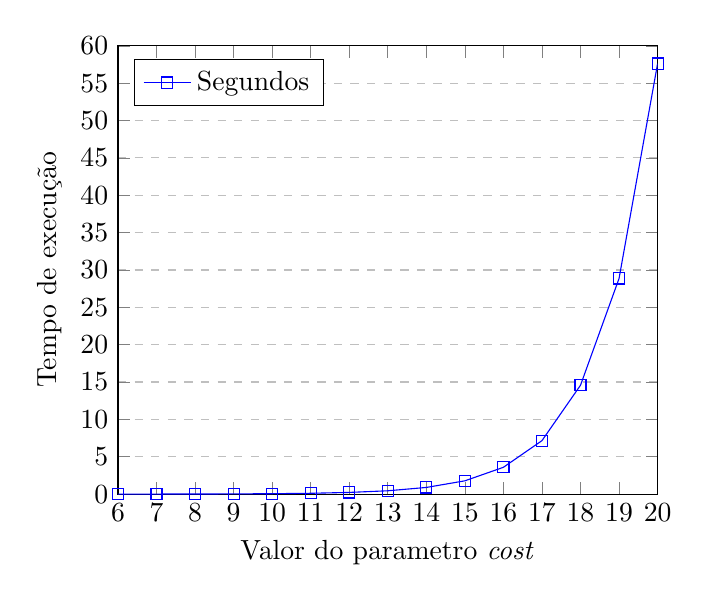
\begin{tikzpicture} 
        \begin{axis}[
            xlabel={Valor do parametro \emph{cost}},
            ylabel={Tempo de execução},
            xmin=6, xmax=20,
            ymin=0, ymax=60,
            xtick={6,7,8,9,10,11,12,13,14,15,16,17,18,19,20},
            ytick={0,5,10,15,20,25,30,35,40,45,50,55,60},
            legend pos=north west,
            ymajorgrids=true,
            grid style=dashed,
        ]
        \addplot[
            color=blue,
            mark=square,
            ]
            coordinates {
            (6,0.003622)(7,0.007590)(8,0.013918)(9,0.028723)(10,0.055023)(11,0.110837)(12,0.226982)(13,0.446507)(14,0.892617)(15,1.778647)(16,3.588397)(17,7.155973)(18,14.572114)(19,28.860461)(20,57.623139)
            };
            \legend{Segundos}
        \end{axis}
    \end{tikzpicture}
\end{center}

%\cleardoublepage
\subsection{bcrypt no mundo real}

Como foi mencionado nas secções prévias, um dos factos de o \emph{bcrypt} ainda ser utilizado deve-se não só à sua segurança, mas ao facto de acompanhar as evoluções tecnológicas a nível de processamento.

Quando foi originalmente lançado em 1999, devido ao tempo de execução do algoritmo \emph{bcrypt} ser adaptável, começou por ser utilizado um fator de custo de 6, pois este era o valor para o qual resultava um tempo de execução de aproximadamente 250ms (considerado por muitos o \emph{standard}).

Devido a enormes avanços tecnológicos, hoje em dia um fator de custo 6 na máquina previamente descrita leva a um tempo de execução de apenas 3.6ms, ou seja, aproximadamente 70 vezes menor do que em 1999.

Para combater esta crescente incessável de poder computacional, o fator de custo deve ser ajustado de acordo com o hardware atual, sendo que hoje em dia o fator de custo mais comum é de 12 a 14, o que nosso teste levou a um tempo de execução entre 226ms e 890ms.

De modo a exemplificar a importância do fator de custo, vamos imaginar o seguinte cenário:

\begin{itemize}
    \item Aplicação com 1000 utilizadores, cujas passwords estão contida num dos conjuntos em baixo especificados.
    \item Conjunto de passwords mais usadas:
    \begin{enumerate}
        \item 100 passwords.
        \item 1000 passwords.
        \item 10000 passwords.
    \end{enumerate}
    \item É permitido tentativas de autenticação ilimitadas, eliminando assim qualquer defesa contra ataques \emph{bruteforce}.
\end{itemize}

Quanto tempo demoraria a um atacante, com um processador idêntico ao descrito anteriormente, testar todas as passwords para os 1000 utilizadores?

\begin{center}
    \begin{tabular}{ |p{2.5cm}|p{3cm}|p{3cm}|p{3cm}|  }
        \hline
        \multicolumn{4}{|c|}{Tempo necessário para testar todas as passwords para os 1000 utilizadores.} \\
        \hline
        Fator de custo & 100 passwords & 1000 passwords & 10000 passwords\\
        \hline 
        6 & 6 minutos & 1 hora & 10 horas\\
        7 & 12 minutos & 2 horas & 21 horas\\
        8 & 23 minutos & 4 horas & 2 dias\\
        9 & 48 minutos & 8 horas & 3 dias\\
        10 & 92 minutos & 15 horas & 6 dias\\
        11 & 3 horas & 30 horas & 13 dias\\
        12 & 6 horas & 3 dias & 1 mês\\
        13 & 12 horas & 5 dias & 2 meses\\
        14 & 1 dia & 10 dias & 3 meses\\
        15 & 2 dias & 21 dias & 7 meses\\
        16 & 4 dias & 1 mês & 1 ano\\
        17 & 1 semana & 3 meses & 2 anos\\
        18 & 2 semanas & 6 meses & 5 anos\\
        19 & 1 mês & 11 meses & 9 anos\\
        20 & 2 meses & 2 anos & 18 anos\\
        \hline
    \end{tabular}
\captionof{table}{Tempo necessário para testar combinações de passwords para 1000 utilizadores.}\label{tab:bcrypt_bruteforce} 
\end{center}

Facilmente percebemos que fatores de custo como 10 são demasiado baixos para a atualidade, sendo imperativo a escolha de um fator de custo equilibrado. Outro facto a ter em consideração é este teste ter sido feito com um processador \emph{mainstream}, sendo que o mesmo se encontra 4 gerações atrasado em comparação com a atual 9ª geração de processadores Intel.

Outro problema que tem ganho tração nos últimos anos, é o aparecimento de soluções especializadas sobre a forma de \gls{gpu}, \gls{fpga}\cite{wiemer2014high}\cite{malvoni2014your} e \gls{asic}, capazes de poder computacional extremamente superior, quando comparados com o \gls{cpu} utilizado para os testes anteriores.

Um \gls{fpga} é um circuito integrado que tem a possibilidade de ser reprogramado através de \emph{bitstreams}, de modo a ser utilizado em aplicações diferentes, como por exemplo, cálculos de hash baseados no algoritmo SHA-1, SHA-256, etc. Enquanto que um \gls{asic}, embora também seja um circuito integrado, apenas consegue fazer uma função e não pode ser reprogramado, no entanto oferece performance muito superior a um \gls{fpga}.

Na tabela \ref{tab:bcrypt_hashrate} exploramos a performance em hashes por segundo (H/s) entre \gls{cpu}\footnote{\gls{cpu} fabricado pela Intel, desenvolvido na arquitetura \emph{Sandy Bridge}.}, \gls{gpu}\footnote{\gls{gpu} fabricada pela NVIDIA, desenvolvida na arquitetura \emph{Maxwell}.} e \gls{fpga}\footnote{Ambos os \gls{fpga} utilizados para comparação são desenvolvidos pela Xilinx.} relativamente ao algoritmo \emph{bcrypt}.

\begin{center}
    \begin{tabular}{ |p{1cm}|p{2.5cm}|p{2cm}|p{2cm}|p{1.75cm}|p{0.9cm}|  }
        \hline
        \multicolumn{6}{|c|}{Cálculo de hashes por segundo (H/s) em diverso hardware.} \\
        \hline
        Tipo & Modelo & Custo 6 & Custo 12 & Consumo & Preço\\
        \hline
        CPU & Xeon E3-1240 & 6210 H/s & 50 H/s& 300W & 262\$\\
        GPU & GTX 750Ti & 1920 H/s& 15 H/s& 300W & 120\$\\
        FPGA & zedboard & 6511 H/s & 51.95 H/s& 4.2W & 319\$\\
        FPGA & Virtex-7 & 51437 H/s& 410.4 H/s& 20W & 3495\$\\
        \hline
    \end{tabular}
\captionof{table}{Comparação entre hardware no cálculo de H/s, eficiência e custo.\cite{wiemer2014high}}\label{tab:bcrypt_hashrate} 
\end{center}

Mais uma vez é possível identificar outro um problema que não foi previamente considerado: como ajustar o fator de custo para este tipo de hardware especializado, como por exemplo \gls{fpga} e \gls{asic}?

Infelizmente a resposta é que este ajuste é deveras impossível. O simples aumento do fator de custo é impensável, pois iria implicar tempos exponenciais de computação em \gls{cpu} mainstream.

Felizmente, tal aplicação de hardware pare este efeito ainda não foi detetada no mundo real e não aparenta qualquer problema de momento.

\cleardoublepage
\section{Autenticação de utilizadores}
A autenticação e gestão de utilizadores é feita através da combinação do middleware\footnote{Middleware é um software que funciona como intermediário entre dois programas.} designado por \emph{Passport} e a base de dados não-relacional\footnote{Estilo de base de dados livres de esquema, capazes de maior escalabilidade que as base de dados tradicionais.} implementada em \emph{MongoDB}.

Devido à informação sensível que pode ser guardada na mesma, campos como a password são, naturalmente, encriptados recorrendo à técnica discutida na secção \ref{encryption}.

%\subsubsection{Passport}
O \emph{Passport} é um middleware de autenticação, desenvolvido para \emph{NodeJS}, com mais de 500 estratégias\footnote{Uma estratégia pode ser interpretado como um mecanismo único de autenticação.} diferentes de autenticação. Foi criado para solucionar um único problema: \textbf{autenticar pedidos}.

Devido à natureza do \emph{Passport}, este é extremamente fácil de implementar numa dada aplicação, devido ao seu forte encapsulamento e ao facto de delegar qualquer funcionalidade, que não seja a autenticação, para a aplicação.

Devido à natureza das aplicações Web modernas, a autenticação pode ser feita por diversas estratégias. As estratégias exploradas neste projeto recairam sobre a escolha mais "tradicional", uma autenticação local com campos para \emph{username} e \emph{password} e a autenticação com o auxílio da ferramenta Autenticação.Gov.

\begin{figure}[h!]
    \centering
    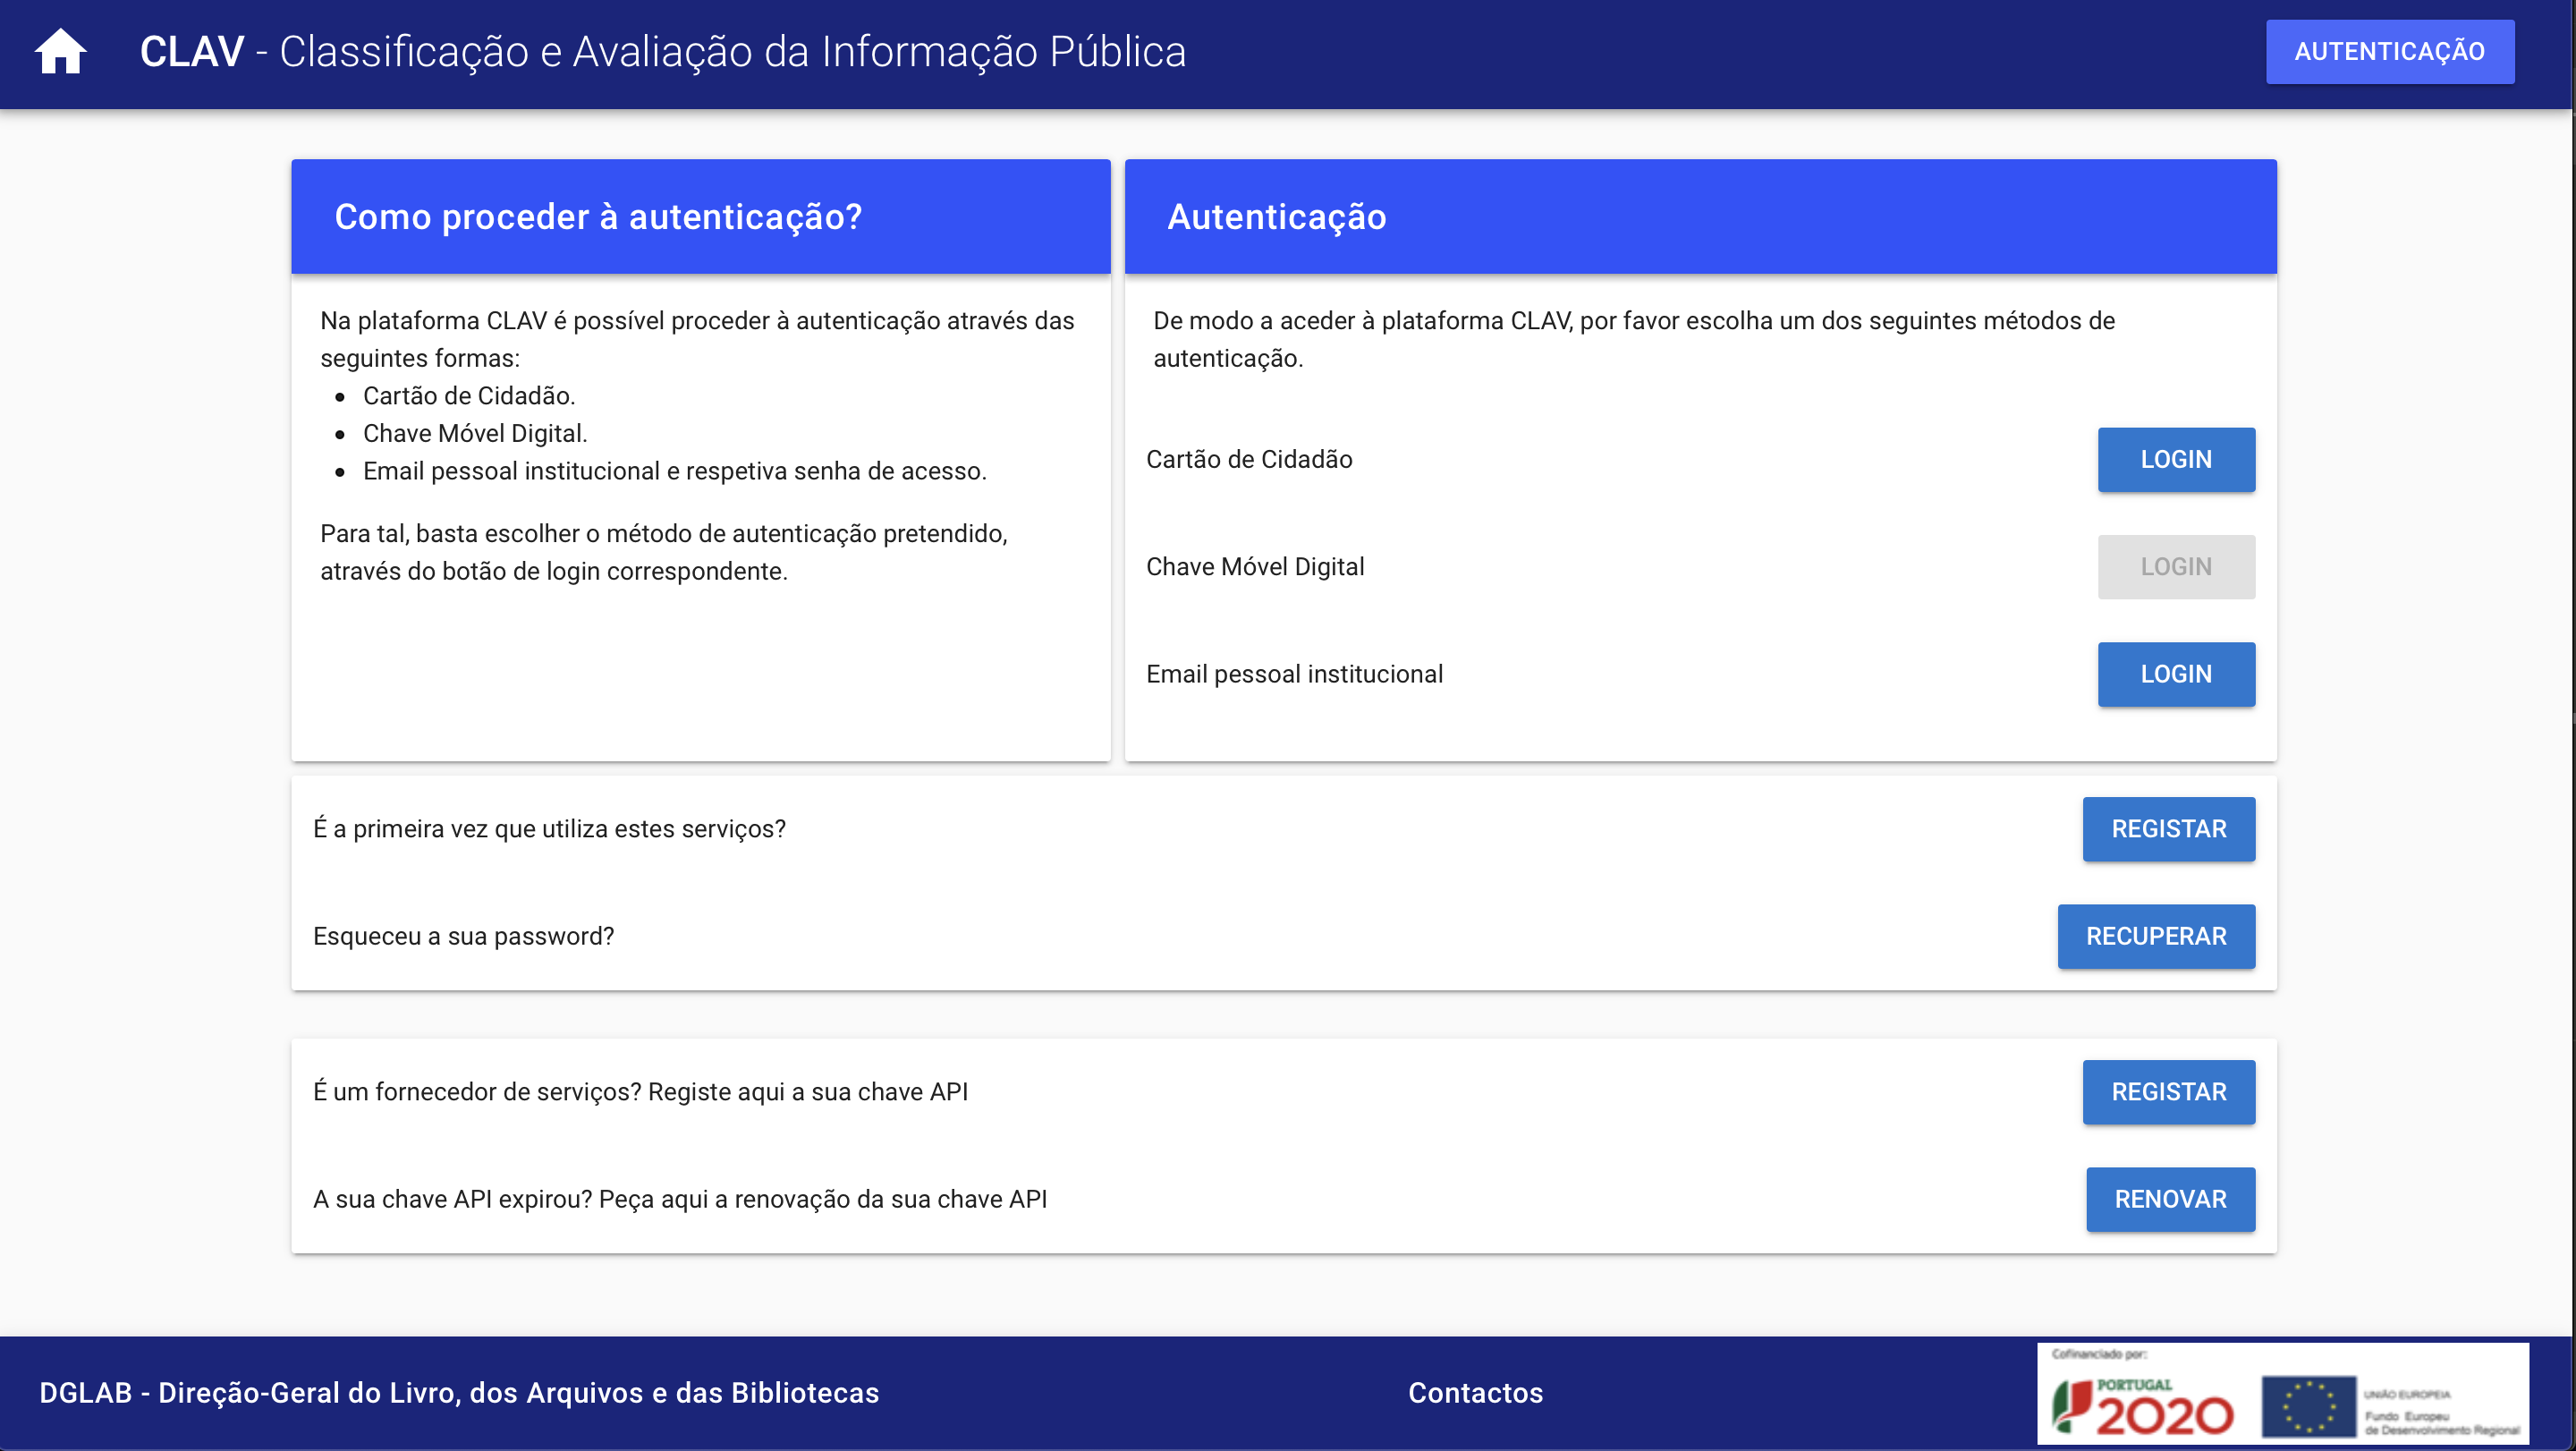
\includegraphics[width=\textwidth]{img/clav/paginaAuth.png}
    \caption{Página responsável pela autenticação na plataforma \gls{clav}.}
    \label{fig:paginaAutenticacao}
\end{figure}

Embora exista um aumento exponencial de implementações de autenticação baseadas em redes sociais, através de protocolos desenvolvidos em acordo com o \emph{OAuth}\footnote{Protocolo open-source que permite autenticação de forma standard e segura, entre aplicações desktop, web e mobile.}, tais como \emph{Google+} e \emph{Facebook}, foi decidido desde uma fase inicial que tais estratégias não seriam consideradas devido ao carácter profissional da plataforma.

Devido a cada aplicação possuir necessidades diferentes, o \emph{Passport} guarda cada estratégia de autenticação em módulos independentes, deixando assim a cargo do programador que estratégias empregar, sem criar dependências desnecessárias.

\subsection{Autenticação através de username e password}



\cleardoublepage
\subsection{Autenticação através de Cartão de Cidadão}

\cleardoublepage
\subsection{Armazenamento e validação de sessões}

De modo a fazer uma gestão de utilizadores mais aprofundada, foi necessário implementar métodos capazes de não só limitar o número de utilizadores ativos a cada dado momento, mas também manter as sessões iniciadas no caso de falha do servidor.

Numa primeira fase do projeto \gls{clav} foi implementada uma solução baseada em \emph{JSON Web Token}, que será explicada na subsecção \ref{jwt_1}. Embora esta se tenha provado eficaz, a mesma não era capaz de manter as sessões iniciadas no caso de uma falha súbita do servidor, ou seja, se o servidor por algum motivo sofresse de uma falha de energia e tivesse de reiniciar, devido às sessões estarem guardadas localmente, as mesmas eram perdidas.

Outro fator decisivo contra esta implementação assenta no facto de não ser possível recorrer ao paralelismo da aplicação através do \emph{nginx}\footnote{Mais informação em \url{https://www.nginx.com}}, pois a comunicação entre processos paralelos não permite a partilha do token guardado localmente.

Para tal, foi necessário recorrer a outra abordagem, o armazenamento de sessões em base de dados, neste caso em \emph{MongoDB}.

\subsubsection{Validação através de JSON Web Token} \label{jwt_1}

Durante o desenvolvimento do projeto \gls{clav} foi discutida a implementação de um mecanismo capaz de terminar sessões automaticamente, de modo a diminuir o número de sessões ativas, bem como evitar possíveis falhas de segurança.

Para tal foi implementado, juntamente com o \emph{Passport}, uma estratégia capaz de lidar com \gls{jwt}, representada através do seguinte pseudo código.

\begin{algorithm}
    \caption{Pseudo código da autenticação via \emph{JSON Web Token}.}
    \begin{algorithmic}[1]
        \Function{JwtStrategy}{opts, jwt\_payload, done}
        \State $user \gets findUserByJwt(jwt\_payload.id)$
        \If {$user \neq invalid$}
            \State \textbf{return} done(null, user)
        \Else
            \State \textbf{return} done(null, false)
        \EndIf
    \EndFunction
    \end{algorithmic}
\end{algorithm}

Através do uso do \emph{JSON Web Token}, é possível povoar o atributo \emph{exp} com uma data de expiração, após a qual o token se torna inválido, terminando assim a sessão do utilizador.

Para tal, quando a estratégia de login local do \emph{Passport} é invocada, é necessário proceder à assinatura de um token \gls{jwt} e atribuí-lo à sessão do utilizador atual.

\begin{algorithm}
    \caption{Pseudo código da atribuição de um \gls{jwt} à sessão.}
    \begin{algorithmic}[1]
        \Function{login}{user}
        \State $token \gets jwt.sign({user}, jwt.secret, \{$
        \State \indent $expiresIn : jwt.expiration$
        \State $\}$
        \State $session.token \gets token$
    \EndFunction
    \end{algorithmic}
\end{algorithm}

Os valores de \emph{secret} e \emph{expiration} previamente utilizados são provenientes de um ficheiro externo, no qual designamos a duração (em segundos) em que a sessão está ativa, bem como a chave secreta utilizada para a assinatura.

\begin{verbatim}
    jwt: {
        secret: 'ihfH6Cv4LVD1YoG...vY8XdVch5ebGHTdPMDGHy',
        expiration: 3000 //in seconds
    }
\end{verbatim}

Após corretamente atribuída a sessão a um utilizador, cada vez que o mesmo pretende aceder a páginas restritas, como por exemplo, a adição de entidades à plataforma \gls{clav} é realizada uma chamada ao \emph{middleware} de autenticação \emph{isLoggedIn}, o qual verifica se existe um utilizador com sessão iniciada, bem como se o token do mesmo ainda não expirou, sendo esta lógica representada através do seguinte pseudo código.

\begin{algorithm}
    \caption{Pseudo código da função  de middleware \emph{isLoggedIn}.}
    \begin{algorithmic}[1]
        \Function{isLoggedIn}{req, res, next}
        \If {$req.isAuthenticated()$}
        \State $result \gets jwt.verify(session.token, jwt.secret)$
            \If {$result \neq expired$}
                \State \textbf{return} next()
            \Else
                \State \textbf{return} err
            \EndIf
        \EndIf
    \EndFunction
    \end{algorithmic}
\end{algorithm}

Embora esta implementação do \emph{JSON Web Token} estivesse 100\% funcional, a mesma foi abandonada da gestão de utilizadores por uma alternativa similar, o armazenamento de sessões ativas diretamente na base de dados em \emph{MongoDB}, sendo apenas utilizado o \gls{jwt} na autenticação de pedidos à \gls{api}.

\cleardoublepage
\subsubsection{Armazenamento em MongoDB}

O armazenamento de sessões em \emph{MongoDB} permite uma maior flexibilidade comparativamente com o armazenamento local.

Em primeiro lugar é possível recorrer ao paralelismo da aplicação via \emph{nginx} ou outras soluções similares, pois cada \emph{thread} pode correr independentemente umas da outras e a comunicação entre processos paralelos passa a ser inexistente. Para validar sessões cada \emph{thread} faz uma \emph{query} à base de dados, verificando se a sessão do utilizador é válida.

Permite também que na ocorrência de uma falha súbita do sistema, as informações relativas às sessões não se percam devido a estarem armazenadas em base de dados. Assim sendo, após o \emph{boot} do sistema, os utilizadores continuam com as sessões ativas, algo que não aconteceria se fosse utilizado armazenamento local e validação via \gls{jwt}.

Um possível problema desta solução seria que iríamos delegar o armazenamento das sessões para o lado do servidor, ou seja, se por ventura existissem milhões de sessões armazenadas, iria ser ocupado um tamanho substancial de memória em disco. Para evitar tal problema, é utilizado o módulo \emph{\textbf{connect-mongo}}\footnote{\url{https://github.com/jdesboeufs/connect-mongo}} que permite a auto remoção de sessões expiradas, bem como a atribuição de um tempo máximo após o qual a sessão expira.

Para atingir este objetivo, apenas é necessário adicionar os campos abaixo mencionados à sessão do \emph{ExpressJS}.

\begin{verbatim}
    app.use(session({
        ...
        autoRemove: 'interval',
        autoRemoveInterval: 15, //minutes
        store: new MongoStore({
            url: dataBases.userDB,
            ttl: 1800 //seconds
        })
    }));
\end{verbatim}

Esta configuração do módulo \emph{\textbf{connect-mongo}} faz com que a cada 15 minutos seja invocada a função de remoção de sessões expiradas, sendo que cada sessão apenas é válida durante 1800 segundos, ou seja, 30 minutos.

Em suma, o armazenamento de sessões em base de dados possui todas as qualidades da validação via \emph{JSON Web Token}, oferecendo uma maior flexibilidade e customização, sem impacto na performance do servidor.

\cleardoublepage
\section{Autenticação de pedidos à API de dados}

De modo a proceder à autenticação de pedidos à \gls{api}, irá ser implementado um sistema baseado em \emph{JSON Web Tokens}.

Esta implementação seguirá as normas propostas pelo \emph{"OAuth 2.0 Authorization Framework: Bearer Token Usage"}\cite{rfc6750}, utilizando para o efeito um header HTTP do tipo \emph{Authorization}, com esquema de autenticação \emph{Bearer}\footnote{Mais informação em \url{https://www.iana.org/assignments/http-authschemes/http-authschemes.xhtml}}.

\begin{figure}[h]
    \centering
    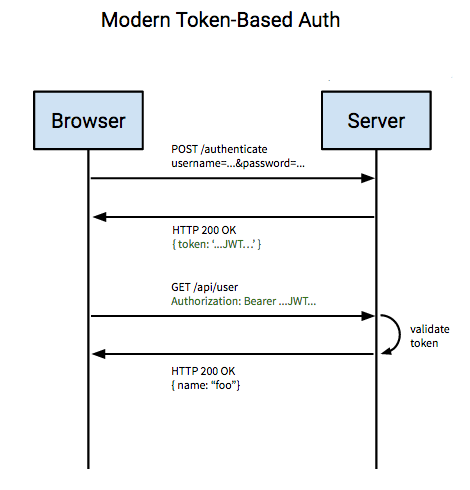
\includegraphics[width=0.75\textwidth]{img/jwt/diagramafluxoJWT.png}
    \caption{Diagrama correspondente à autenticação baseda em tokens. \cite{jwtDiagram}}
\end{figure}

O sistema de autenticação a ser implementado seguirá o diagrama previamente descrito, ou seja:

\begin{enumerate}
    \item É realizada a autenticação de um elemento externo no nosso servidor.
    \item Caso a autenticação tenha sucesso, irá ser devolvido um \gls{jwt} que irá servir de \emph{API Key} para a autenticação de chamadas à mesma.
    \item Cada vez que é feita uma chamada à \gls{api}, o token presente no campo \emph{Authorization} irá ser validado.
    \item Caso este seja validado com sucesso, irá ser retornado o output da chamada à API solicitada.
\end{enumerate}

Outra possibilidade de implementação é descrita a seguir, onde no servidor 3 (neste caso, o servidor responsável por correr o projeto \gls{clav}), possui uma lista de \emph{API Key} válidas (neste caso, \gls{jwt}).

\begin{figure}[h]
    \centering
    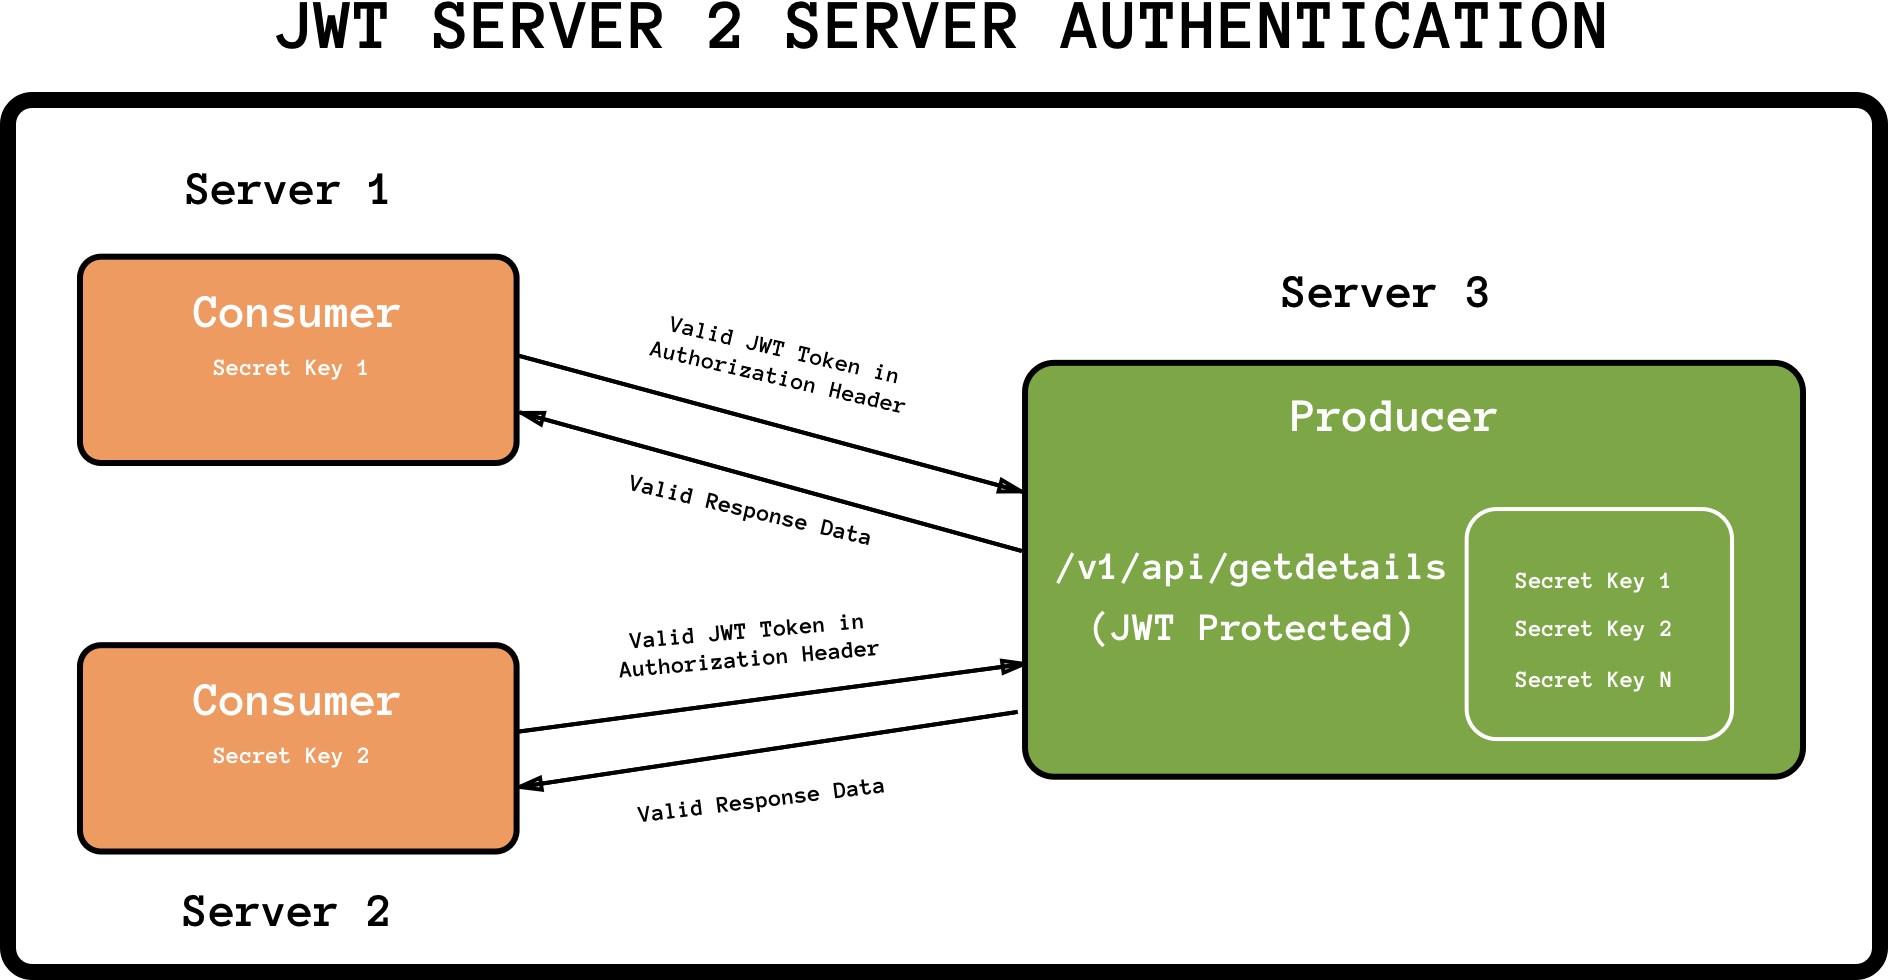
\includegraphics[width=\textwidth]{img/jwt/jwtAPI.png}
    \caption{Representação da utilização de \emph{JSON Web Token} para autenticação de pedidos à API. \cite{jwtAPI}}
\end{figure}

Cada vez que uma chamada à \gls{api} é feita, irá ser verificado se o \emph{token} dos utilizadores (representados por consumidores na imagem), está presente na lista de chaves pré validadas.

\cleardoublepage
\section{Autenticação backend}

De modo a proporcionar mecanismos capazes de lidar com os diversos tipos de utilizadores presentes na plataforma \gls{clav}, foi implementada uma solução baseada em \emph{middleware}. As funções de \emph{middleware} são responsáveis pela verificação do nível de acesso do utilizador. 

Para tal, foram desenvolvidas as seguintes funções, \emph{checkLevel} e \emph{isLevel}, sendo a primeira uma chamada à função auxiliar \emph{isLevel}.

\begin{algorithm}
    \caption{Pseudo código da função de middleware \emph{checkLevel}.}
    \begin{algorithmic}[1]
        \Function{checkLevel7}{user, next}
            \State \textbf{return} isLevel(7, user, next)
    \EndFunction
    \end{algorithmic}
\end{algorithm}

No pseudo código anterior podemos ver a implementação da função \emph{checkLevel7}, cujo objectivo é verificar se o utilizador possui acesso de nível 7, ou superior.

Esta função recorre a uma chamada à função \emph{isLevel}, sendo passado como parâmetro o nível de acesso a verificar.

\begin{algorithm}
    \caption{Pseudo código da função de middleware \emph{isLevel}.}
    \begin{algorithmic}[1]
    \Function{isLevel}{clearance, user, next}
        \If {$user.isAuthenticated$}
            \If {$user.level \geq clearance$}
                \State \textbf{return} next()
            \Else
                \State \textbf{return} redirect('back')
            \EndIf
        \Else
            \State \textbf{return} redirect('login')
        \EndIf
    \EndFunction
    \end{algorithmic}
\end{algorithm}

Com as estratégias de autenticação mencionadas anteriormente podemos assegurar uma correta implementação de níveis de acesso, não sendo possível a utilizadores aceder a conteúdo ao qual não possuem permissão.